% C.10 等腰△，AB=AC, 顶角 A=36°
\documentclass[tikz,border=4pt]{standalone}
\usepackage{ctex}
\usepackage{amsmath}
\usetikzlibrary{calc, arrows.meta,decorations.markings}
\begin{document}
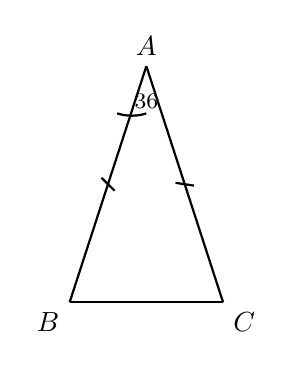
\begin{tikzpicture}[scale=1.0, thick,
  tickone/.style={postaction={decorate, decoration={markings,
    mark=at position 0.5 with {\draw (-1.5pt,-3pt) -- (1.5pt,3pt);}}}}]
  \coordinate (A) at (0,3);
  \pgfmathsetmacro{\hw}{3*tan(18)}
  \coordinate (B) at (-\hw,0);
  \coordinate (C) at (\hw,0);
  \draw[tickone] (A) -- (B);
  \draw[tickone] (A) -- (C);
  \draw (B) -- (C);
  \node[above] at (A) {$A$};
  \node[below left] at (B) {$B$};
  \node[below right] at (C) {$C$};
  \draw (0,2.4) arc (-90+18:-90-18:0.6);
  \node[font=\footnotesize] at (0,2.55) {$36°$};
\end{tikzpicture}
\end{document}
